\documentclass{article}
\usepackage{amsmath}
\usepackage{graphicx}
\usepackage{amssymb}
\usepackage{enumitem}
\usepackage{float}
\usepackage{textcomp,gensymb}
\usepackage[utf8]{inputenc}
\providecommand{\brak}[1]{\ensuremath{\left (#1\right)}}
\providecommand{\sbrak}[1]{\ensuremath{\left[#1\right]}}
\title{Assignment}
\author{CBSE 2017 Mathematics}
\begin{document}
\maketitle
\begin{enumerate}
\section*{Quadratic Equations}
\item Find the value of $p$, for which one root of the equation 
\begin{align*}
	px^2-14x+8=0
\end{align*}
is $6$ times the other.
\item If the roots of the equation
\begin{align*}
	\brak{c^2-ab}x^2-2\brak{a^2-bc}x+b^2-ac=0 
\end{align*}
in x are equal, then show that either a=0 or 
\begin{align*}
	a^3+b^3+c^3=3abc.
\end{align*}
\item Solve for x:
\begin{align*}
\dfrac{1}{2x-3}+\dfrac{1}{x-5}=1\dfrac{1}{9}, x\neq\dfrac{3}{2},5 
\end{align*}
\item A train covers a distance of $300$ km at a uniform speed. If the speed of the train is increased by $5$ km/hour, it takes $2$ hours less in the journey. Find the original speed of the  train.

\section*{Arithmetic Progressions}
\item What is the common difference of an A.P. in which $a_{21}$ - $a_7$ = $84$ ?
\item Which term of the A.P.$8,14,20,26,$\ldots will be $72$ more than its $41^{st}$ term ?

\item If the $10^{th}$ term of an A.P. is $52$ and the $17^{th}$ term is $20$ more than the $13^{th}$ term, find the A.P.
\item If the ratio of the sum of the first n terms of two A.Ps is $\brak{7n + 1}$ : $\brak{4n + 27}$, then find the ratio of their $9^{th}$ terms.

\section*{Triangles}
\item Construct a triangle $ABC$ with side BC = $7$ cm, $\angle{B}$=$45\degree$, $\angle{A}$=$105\degree$. Then construct another triangle whose sides are  $\dfrac{3}{4}$  times the corresponding sides of the $\triangle$ ABC.

\section*{Coordinate Geometry}
\item In what ratio does the point $\brak{\dfrac{24}{11},y}$ divide the line segment joining the points $P\brak{2,-2}$ and $Q\brak{3,7}$ ? Also find the value of $y$.
\item A line intersects the y-axis and x-axis at the points $P$ and $Q$ respectively. If $\brak{2,-5}$ is the mid-point of $PQ$, then find the coordinates of $P$ and $Q$. 
\item If the distances of $P\brak{x,y}$ from $A\brak{5,1}$ and $B\brak{-1,5}$ are equal, then prove that $3x=2y$.
\item If the points $A\brak{k+1, 2k}$, $B\brak{3k, 2k + 3}$  and $C\brak{5k-1, 5k}$ are collinear, then find the value of k.

\section*{Some Applications of trigonometry}
\item If a tower $30$ m high, casts a shadow $10\sqrt{3}$ m long on a ground, then what is the angle of elevation of the sun ?
\item On a straight line passing through the foot of a tower, two points $C$ and $D$ are at distances of $4$ m and $16$ m from the foot respectively. If the angles of elevation from $C$ and $D$ of the top of the tower are complementary, then  find the  height of the tower.
\item A man observes a car from the top of a tower, which is  moving towards the tower with a uniform speed. If the angle of depression of the car changes from $30\degree$ to $45\degree$ in $12$ minutes, find the time taken by the car now to reach the tower.

\section*{Circles}
\item If the angle between two tangents drawn from an external point $P$ to a circle of radius a and centre $O$, is $60\degree$, then find the length of $OP$.
\item Prove that the tangents drawn at the end points of a chord of a circle make equal angles with the chord.
\item A circle touches all the four sides of a quadrilateral $ABCD$. Prove that
\begin{align*}
		AB + CD = BC +DA
\end{align*}
\item Prove that the lengths of two tangents drawn from an external point to a circle are equal.
\item In the given figure, $XY$ and $X\rq Y\rq$ are two parallel tangents to a circle with centre $O$ and another tangent $AB$ with point of contact $C$, is intersecting $XY$ at $A$ and $X\rq Y\rq$ at $B$. Prove that $\angle{AOB}$=90$\degree$.
\begin{figure}[H]
\centering
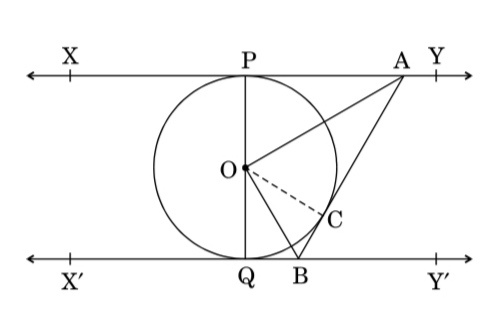
\includegraphics[width=0.8 \columnwidth]{Figs/Fig2.jpg}
\end{figure}

\section*{Areas Related Circles}
\item In the given figure, two concentric circles with  centre $O$ have radii $21$ cm and $42$ cm. If $\angle{AOB}$= $60\degree$, find the area of the shaded region.

\hfill$\sbrak{Use\ \pi = \dfrac{22}{7}}$
\begin{figure}[H]
\centering
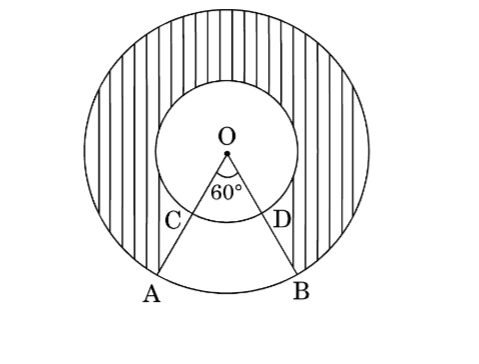
\includegraphics[width=0.8 \columnwidth]{Figs/Fig.jpg}
\end{figure}
\item Three semicircles each of diameter $3$ cm, a circle of diameter $4·5$ cm and a semicircle of radius $4·5$ cm are drawn in the given figure. Find the area of the shaded region.
\begin{figure}[H]
\centering
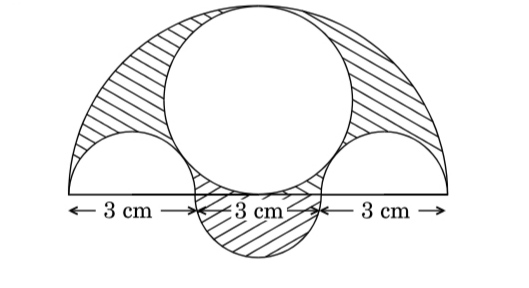
\includegraphics[width=0.8 \columnwidth]{Figs/Fig1.jpg}
\end{figure}
\item In the given figure, $\triangle$ $ABC$ is a right-angled triangle in which $\angle{A}$ = 90$\degree$. Semicircles are drawn on $AB$, $AC$ and $BC$ as diameters. Find the area of the shaded region.
\begin{figure}[H]
\centering
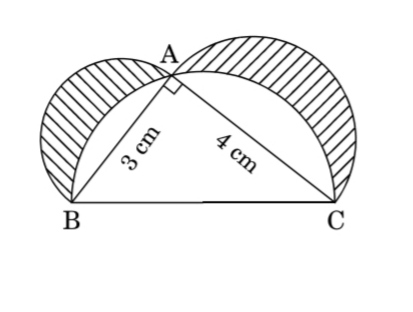
\includegraphics[width=0.8 \columnwidth]{Figs/Fig3.jpg}
\end{figure}

\section*{Surface Areas and Volumes}
\item The dimensions of a solid iron cuboid are $4.4$ m $\times$ $2.6$ m $\times$ $1.0$ m. It is melted and recast into a hollow cylindrical pipe of $30$ cm inner radius and thickness $5$ cm. Find the length of the pipe. 
\item Water in a canal, $5·4$ m wide and $1·8$ m deep, is flowing with a speed of $25$ km/hour. How much area can it irrigate in $40$ minutes, if $10$ cm of standing water is required for irrigation ?
\item From a solid right circular cylinder of height $2·4$ cm and radius $0·7$ cm, a right circular cone of same height and same radius is cut out. Find the total surface area of the remaining solid.
\item In a rain-water harvesting system, the rain-water from aroof of $22 $ m $\times$ $20$ m drains into a cylindrical tank having diameter of base $2$ m  and height $3·5$ m. If the tank is full, find the rainfall in cm. Write your views on water conservation.

\section*{Probability}
\item The probability of selecting a rotten apple randomly from a heap of $900$ apples is $0.18$. What is the number of rotten apples in the heap ?
\item A bag contains $15$ white and some black balls. If the probability of drawing a black ball from the bag is thrice that of drawing a white ball, find the number of blackballs in the bag.
\item Two different dice are thrown together. Find the probability that the numbers obtained have
\begin{enumerate}[label=\roman*]
\item even sum, and
\item even product.
\end{enumerate} 
\end{enumerate}
\end{document}
